% !TEX root = ../main.tex

\chapter{相关工作}

\section{膝关节组织深度学习分割方法}
  近年来，深度学习（Deep Learning, DL）技术在医学图像处理领域取得了较快进展，
  尤其是卷积神经网络（Convolutional Neural Network, CNN）在膝关节磁共振图像（MRI）分割中展现出较好的性能。
  准确分割膝关节的关键组织（如关节软骨、半月板、韧带和骨骼）对于骨关节炎等疾病的定量分析与辅助诊断至关重要。
  目前，基于U-Net和V-Net架构及其衍生变体的深度学习方法构成了该领域的研究主流。
  \subsection{U-Net架构及其在膝关节二维分割中的应用}
    U-Net 由 Ronneberger 等人于2015年首次提出，其最显著的特征是对称的“编码器-解码器（Encoder-Decoder）”U型结构以及跳跃连接（Skip Connections）机制\cite{ronnebergerUNetConvolutionalNetworks2015c}。
    编码器通过连续的卷积与下采样操作提取图像的高维抽象语义特征，而解码器则通过上采样逐步恢复图像的空间分辨率。
    跳跃连接巧妙地将编码器中保留了丰富空间位置信息的浅层特征图与解码器中的深层语义特征图在通道维度上进行拼接，从而有效解决了医学图像中边界模糊、目标细小的问题。
    \begin{figure}[!htp]
      \centering
      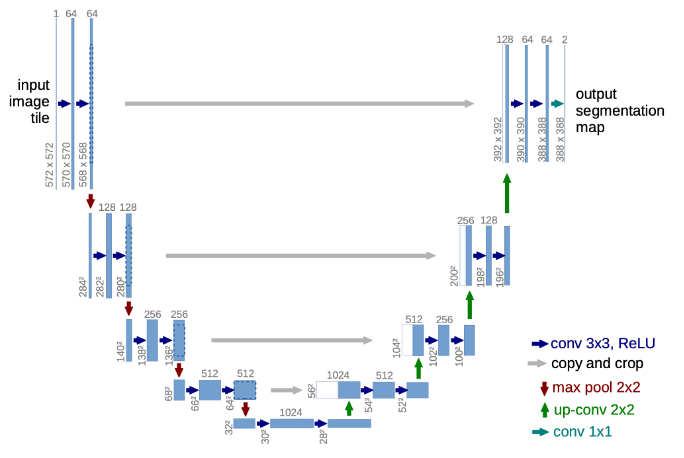
\includegraphics[width=0.8\linewidth]{figures/unet.png}
      \caption{U-Net架构示意图。图片来源：Ronneberger 等人\cite{ronnebergerUNetConvolutionalNetworks2015c}。}
      \label{fig:unet}
    \end{figure}
    \par 在膝关节MRI的分割应用中，由于软骨呈现较薄的曲面分布，U-Net展现出较好的边界还原能力。
    例如，Norman 等人利用 2D U-Net 卷积神经网络对膝关节MRI数据进行了自动化的软骨和半月板分割，为后续的形态学与弛豫时间（Relaxometry）定量分析提供了掩膜基础\cite{bUse2DUNet2018}。
  \subsection{面向三维体积的V-Net与损失函数优化}
    由于临床膝关节MRI数据（如DESS或FSE序列）通常是具有层间物理间距的三维体积数据，直接对其进行逐层2D分割会割裂Z轴方向上的解剖连续性。
    为解决这一问题，Milletari 等人提出了完全基于三维卷积的 V-Net 架构\cite{milletariVNetFullyConvolutional2016a}。
    V-Net 继承了 U-Net 的整体拓扑，但将所有的2D操作升级为3D操作，并在卷积块中引入了残差学习（Residual Learning）以加速网络收敛。
    \par 此外，V-Net 在医学图像分割领域的一个重要贡献是较早系统采用了基于 Dice 相似系数的损失函数（Dice Loss）。
    在膝关节影像中，软骨与骨髓病变（BML）的体素数量往往远少于背景及其他组织，存在明显的类别不平衡（Class Imbalance）问题。
    传统的交叉熵损失会主导网络偏向于预测背景，而 Dice 损失通过全局计算预测掩膜与真实标签的重叠率，在一定程度上提升了网络对软骨等小目标结构的分割灵敏度。
  \subsection{网络变体、自适应框架与多平面策略}
    随着算法的演进，研究者在基础 U-Net 的框架上衍生出了众多变体\cite{kesslerOptimisationDeepNeural2020}。
    例如，研究表明基于 SegNet 变体的编解码器架构在骨与软骨的分割中同样能够实现较好的特征还原。
    近年来，Isensee 等人提出的 nnU-Net（No-New-Net）框架通过自适应配置预处理、网络拓扑及后处理策略，在包括膝关节在内的多项医学图像分割任务中确立了重要的性能基准\cite{isenseeNnUNetSelfconfiguringMethod2021}。
    \par 然而，在处理高分辨率膝关节三维MRI时，直接采用全3D网络（如3D U-Net）面临着较大的图形处理器（Graphics Processing Unit, GPU）显存开销限制，而传统的单平面2D网络又缺乏空间上下文信息。
    因此，“2.5D切片融合”与“多平面网络（Multi-Planar Networks）”成为平衡计算成本与分割精度的重要方向。
    例如，Multi-Planar U-Net 等架构通过将包含目标体素的二维切片沿矢状面、冠状面和轴状面（Sagittal, Coronal, Axial）三个正交视角分别提取并输入平行的 2D 网络，最后在输出端进行多视角预测特征的三维融合（Multi-view Fusion）\cite{ryuMultiplanar25DUNet2023} 。

\section{医学图像的域适应技术}
  \subsection{基于图像翻译的生成式模型 CycleGAN}
    图像翻译（Image Translation）是图像域适应领域（Domain Adaptation, DA） 的重要分支。其中大部分技术都需要成对的训练数据，但这在医学图像领域非常稀缺。
    CycleGAN（Cycle-Consistent Adversarial Networks）\cite{zhuUnpairedImagetoImageTranslation2017}凭借无需成对的训练数据的特性，被广泛应用在跨模态或跨中心的医学影像迁移（如 MRI 到计算机断层扫描（Computed Tomography, CT）\cite{wolterinkDeepMRCT2017a}）。
    该模型通过引入循环一致性损失（Cycle-consistency Loss），约束了源域图像在经过双向映射后能够回到原始状态，从而实现了非成对数据上的风格迁移。
    \begin{figure}[!htp]
      \centering
      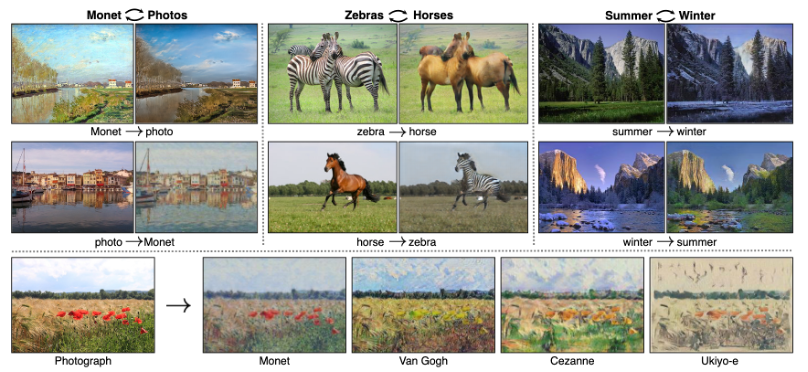
\includegraphics[width=0.8\linewidth]{figures/cyclegan.png}
      \caption{CycleGAN架构示意图。图片来源：Zhu 等人\cite{zhuUnpairedImagetoImageTranslation2017}。}
      \label{fig:cyclegan}
    \end{figure}
    \subsubsection{核心挑战}
      无配对数据域迁移的主要挑战在于，单向的映射 $G:X \to Y$ 是高度欠约束的，存在多种映射方式可以使输出分布与目标分布相同，这可能导致“模式崩溃（Mode Collapse）”的问题，即所有输入都被映射到同一张输出图像上。
    \subsubsection{核心架构设计}
      为了解决上述欠约束问题，CycleGAN 引入了两个映射函数和两个判别器，并结合了“循环一致性”的结构假设。
      双生成器（映射函数）：
      \begin{itemize}
        \item 生成器 $G$：负责将图像从域 X 转换到域 Y（即 $G:X \to Y$）。
        \item 生成器 $F$：负责将图像从域 Y 转换回域 X（即 $F:Y \to X$）。
      \end{itemize}
      双判别器：
      \begin{itemize}
        \item 判别器 $D_Y$：用于区分真实的 $Y$ 域图像 $y$ 和生成的图像 $G(x)$ 。
        \item 判别器 $D_X$：用于区分真实的 $X$ 域图像 $x$ 和生成的图像 $F(y)$ 。
      \end{itemize}
    \subsubsection{关键损失函数}
      对抗损失（Adversarial Loss）：
      用于确保生成的图像在分布上与目标域的真实图像无法区分。以从 $X$ 到 $Y$ 的映射为例，生成器 $G$ 试图最小化该损失，而判别器 $D_Y$ 试图最大化该损失：
      \begin{equation}
        \mathcal{L}_{GAN}(G, D_Y, X, Y) = \mathbb{E}_{y \sim p_{data}(y)} [\log D_Y(y)] + \mathbb{E}_{x \sim p_{data}(x)} [\log (1 - D_Y(G(x)))].
      \end{equation}
      同理，反向映射也具有对应的对抗损失：
      \begin{equation}
        \mathcal{L}_{GAN}(F, D_X, Y, X) = \mathbb{E}_{x \sim p_{data}(x)} [\log D_X(x)] + \mathbb{E}_{y \sim p_{data}(y)} [\log (1 - D_X(F(y)))].
      \end{equation}
      循环一致性损失（Cycle Consistency Loss）：
      为了防止生成器将输入图像随机排列映射到目标域中，该损失强制要求翻译过程具有可逆性 ：
      \begin{itemize}
        \item 前向循环一致性：$x \to G(x) \to F(G(x)) \approx x$。
        \item 反向循环一致性：$y \to F(y) \to G(F(y)) \approx y$。
      \end{itemize}
      该损失通过计算重构图像与原输入图像之间的 L1 范数距离来实现：
      \begin{equation}
        \mathcal{L}_{cyc}(G, F) = \mathbb{E}_{x \sim p_{data}(x)} [\| F(G(x)) - x \|_1] + \mathbb{E}_{y \sim p_{data}(y)} [\| G(F(y)) - y \|_1].
      \end{equation}
    \subsubsection{总体优化目标}
      最终的总目标函数是上述损失的加权组合：
      \begin{equation}
        \mathcal{L}(G, F, D_X, D_Y) = \mathcal{L}_{GAN}(G, D_Y, X, Y) + \mathcal{L}_{GAN}(F, D_X, Y, X) + \lambda \mathcal{L}_{cyc}(G, F),
      \end{equation}
      模型通过求解 $\min_{G,F} \max_{D_X,D_Y} \mathcal{L}(G, F, D_X, D_Y)$ 来寻找最优生成器和判别器权重。
    \subsubsection{在骨关节医学影像领域的应用}
      在骨关节医学影像领域，也有研究尝试利用 CycleGAN 缩小不同数据集之间的风格差异。
      Felfeliyan et al. 利用 CycleGAN 将 OAI 数据集中的 TSE（Turbo Spin Echo） 序列转换为 DESS（Double Echo Steady State） 序列，
      以实现无监督的软骨和骨骼分割\cite{felfeliyanMRIKneeDomain2021}。
      \par 然而，在实际操作过程中，由于 CycleGAN 缺乏对局部精细解剖结构的强约束，往往会导致膝关节的细小韧带结构、软骨和骨骼的边缘发生扭曲，造成结构畸变。
      同时，ACL 损伤相关的病理特征（如 BML 信号）在风格迁移过程中可能被视为噪声后抹除，或者引入不真实的伪影，从而影响后续针对 BML 临床指标的下游定量分析。
  \subsection{基于特征对齐的模型 DANN}
    \subsubsection{研究背景与核心理论}
      在机器学习中，由于获取目标域（Target Domain）的标注数据成本高昂，
      通常需要在包含标注数据的源域（Source Domain）上训练模型，并试图将其应用到无标注的目标域中。
      然而，这两个域之间往往存在数据分布的偏移（Distribution Shift）。
      \par 域对抗神经网络（Domain-Adversarial Neural Networks, DANN）\cite{ganinDomainAdversarialTrainingNeural2017}的核心理论基础是 Ben-David 等人提出的H-散度理论\cite{ben-davidTheoryLearningDifferent2010}。
      该理论指出：如果一个学习算法无法识别输入数据是来自源域还是目标域，那么这种特征表示对于跨域迁移就是有效的。
    \subsubsection{核心架构设计}
      DANN 将领域自适应与深度特征学习无缝融合在同一个训练过程中 ，其网络架构主要由三个关键部分组成：
      \begin{itemize}
        \item 特征提取器（Feature Extractor）$G_f$：负责从输入数据中提取高维特征表示。
        \item 标签分类器（Label Classifier）$G_y$：基于特征提取器输出的特征进行标签预测，训练目标是最小化源域上的分类损失。
        \item 域分类器（Domain Classifier）$G_d$：用于区分输入数据来自源域还是目标域，训练目标是最大化该分类损失，以使特征提取器学习到对域不可区分的特征表示。
      \end{itemize}
    \subsubsection{梯度反转层}
      DANN 的最大技术创新在于引入了一个梯度反转层（Gradient Reversal Layer, GRL），它被放置在特征提取器 $G_f$ 和域分类器 $G_d$ 之间。
      \begin{itemize}
        \item 前向传播（Forward Propagation）：GRL 作为一个恒等变换不改变数据，直接将特征传递给域分类器。
        \item 反向传播（Backpropagation）：GRL 会将从域分类器传回的梯度乘以一个负常数（改变梯度的符号），然后再传递给底层的特征提取器。
      \end{itemize}
      \par 这一设计非常巧妙，使得原本基于反向传播的随机梯度下降算法（Stochastic Gradient Descent, SGD），
      能够直接用于求解原本复杂的对抗性的 Min-Max 优化问题。
    \subsubsection{总体优化目标与博弈过程}
      DANN 的优化目标是寻找一个鞍点（Saddle Point），使得特征提取器和标签预测器联合最小化分类误差，同时特征提取器又要最大化域分类器的误差。
      \par 具体而言，模型优化以下总目标函数：
      \begin{equation}
        E\left(\theta_f, \theta_y, \theta_d\right)=\frac{1}{n} \sum_{i=1}^n \mathcal{L}_y^i\left(\theta_f, \theta_y\right)-\lambda\left(\frac{1}{n} \sum_{i=1}^n \mathcal{L}_d^i\left(\theta_f, \theta_d\right)+\frac{1}{n^{\prime}} \sum_{i=n+1}^N \mathcal{L}_d^i\left(\theta_f, \theta_d\right)\right)
      \end{equation}
      对于标签预测器参数 $\theta_y$ 和域分类器参数 $\theta_d$：
      按照常规梯度下降方向更新，分别最小化各自的损失（分类损失 $L_y$ 和领域判别损失 $L_d$）。
      \par 对于特征提取器参数 $\theta_f$：需要最小化标签预测损失 $L_y$，但通过 GRL 的负号作用，实质上是在最大化领域判别损失 $L_d$。

\section{多视图MRI融合与超分辨率重建}
  在膝关节的临床影像学检查中，由于成像时间与信噪比（SNR）的限制，常规的二维快速自旋回波（2D FSE）序列通常具有较高的面内分辨率，
  但在层厚方向（Z轴）上往往需要设定较厚的切片间距（例如2至4毫米）。
  这种各向异性（Anisotropic）的体素分布会导致较明显的部分容积效应（Partial Volume Effects），
  使得图像无法在任意平面上进行高质量的多平面重组，从而限制了对较薄关节软骨进行精确三维形态学评估与体积、厚度测量。
  为了缓解这一物理扫描限制，多视图融合与超分辨率重建（Super-Resolution Reconstruction, SRR）技术逐渐受到关注\cite{lomurnoImprovingMultiViewStereo2022}。
  \subsection{图像超分辨率与切片到体积重构（SVR）原理}
    超分辨率重建技术的核心思想是通过算法从低分辨率（Low-resolution）或欠采样的数据中恢复出高质量的高分辨率（High-resolution）图像细节。
    其中，切片到体积重构（Slice-to-Volume Reconstruction, SVR）是医学图像超分辨率领域的一项关键技术。
    SVR最初被广泛应用于胎儿MRI领域，以解决由于胎儿及母体运动导致的层间伪影问题，其通过快速采集较厚的2D切片来冻结面内运动\cite{jiangMRIMovingSubjects2007}，随后利用算法在三维空间中恢复解剖结构。
    \par 传统的SVR方法将体积重建建模为一个联合配准与超分辨率的逆问题（Inverse problem）。
    算法通过建立切片采集的数学模型，迭代地估计二维切片到三维体积的空间变换矩阵，并优化重构出高分辨率的三维体素强度\cite{gholipourRobustSuperresolutionVolume2010}。
    这种基于物理模型的重构技术能够有效地将离散的二维信息映射到连续的三维网格上。
  \subsection{跨正交平面的信息互补与融合}
    对于膝关节这种具有复杂拓扑结构的运动器官，单一的扫描平面不可避免地存在视觉盲区。
    然而，临床上常规采集的矢状面（Sagittal）、冠状面（Coronal）和轴状面（Axial）三个正交视角之间蕴含着丰富的互补空间信息。
    通过将这三个视角的各向异性数据集联合起来，可以利用它们在交叉区域的重叠信息，精确推断出潜在的三维结构。
  \subsection{基于刚性配准与深度图像先验（DIP）的无监督多视图融合重建}
    在临床磁共振成像中，为了在有限的扫描时间内抑制运动伪影并保证信噪比（SNR），通常会采用二维厚层采集（如常规FSE序列），
    这导致了图像在层内具有较高分辨率，而在层间方向分辨率较低。
    为了从这些各向异性（Anisotropic）的二维切片中恢复出各向同性（Isotropic）的三维解剖结构，
    多视图切片到体积重建（Slice-to-Volume Reconstruction, SVR）技术成为了研究热点。
    \subsubsection{传统SVR方法与多视图优化的局限性}
      传统的SVR方法通常将体积重建建模为一个联合配准与超分辨率的逆问题（Inverse problem）。
      以领域内广泛使用的开源工具NiftyMIC为例，其核心工作流依赖于两步迭代法：
      交替进行刚性切片到体积的配准（Rigid slice-to-volume registration）与超分辨率重建（SRR）循环\cite{ebnerAutomatedFrameworkLocalization2020}。
      尽管这类基于物理优化模型的方法在处理胎儿或新生儿MRI的运动伪影中取得了成效，但其本质上依赖于离散的体素网格表示。
      这种离散化不仅导致计算复杂度和内存消耗随体积大小快速增长，而且在面对形态较复杂的膝关节软骨时，容易在正交平面的交叉处产生网格状伪影。
    \subsubsection{深度学习的引入与监督数据的瓶颈}
      将卷积神经网络（CNN）引入到超分辨率重建中，能够减轻传统优化的计算负担情况。但是绝大多数现有的深度学习超分辨率模型都是监督学习，
      训练通常依赖于大量且精确对齐的高分辨率与低分辨率图像对（HR-LR pairs）。
      在真实的膝关节临床扫描中，由于患者的微小运动，获取精确对齐的多平面各向同性高保真金标准存在较大困难。
      这种监督数据的缺失会因此导致常规深度学习模型在实际应用中，面临过拟合风险和跨域测试时的光谱伪影。
    \subsubsection{深度图像先验（DIP）的无监督范式转换}
      为了降低监督学习对成对数据的依赖，Ulyanov等人提出了一种无监督框架——深度图像先验（Deep Image Prior, DIP）。
      该理论认为，卷积神经网络自身的拓扑架构（如U-Net）在随机初始化状态下，也会体现一定的底层图像统计先验信息。
      DIP不需要外部成对的训练数据，可以利用输入的退化图像进行从头优化（De novo optimization）\cite{ulyanovDeepImagePrior2020}。
      \par 在MRI超分辨率重建任务中，DIP会把一个随机初始化的网络作为先验约束器，然后通过定义一个模拟切片降采样的前向物理退化模型，
      来迭代最小化网络生成的三维体积与输入的各向异性的二维切片之间的重建损失。
      在此过程中网络可被视为一种隐式的平滑与锐化正则化器（Regularizer）。
      因为DIP在优化过程中天然地抗拒高频噪声而倾向于拟合自然解剖的低频连续结构，
      所以它有潜力融合来自矢状、冠状和轴状三个正交视角的互补信息。
      \par 综上所述，DIP技术为医学图像的无监督多视图超分辨率重建提供了一条无需外部标签的候选路径。
      它在减少跨平面层间断层伪影、恢复平滑解剖边界方面具有一定潜力，
      为本文在研究局限性与未来工作中讨论基于配准联合DIP的膝关节候选融合方向提供了理论参考。

\section{现有研究的不足与本文切入点}
  综合上述文献分析，目前针对膝关节医学影像的深度学习分割与重建技术虽已取得一定进展，但在应对真实临床环境时仍存在以下主要问题：
  \begin{itemize}
    \item 依赖强监督范式：主流的U-Net、V-Net等模型通常需要大规模且精确配对的体素级标注数据。这种强监督范式获取成本较高，且难以覆盖临床真实场景中复杂多样的病理变异。
    \item 生成式域适应可能影响解剖保真度：在解决数据域分布偏移时，当前部分研究倾向于使用CycleGAN等基于图像翻译的无监督方法。然而，此类生成式模型缺乏对局部关键解剖结构拓扑的直接约束，在跨序列翻译过程中可能产生“幻构”伪影，甚至抹除BML等隐匿的病理高信号，影响后续临床定量分析的可靠性。
    \item 传统三维重建方法计算开销较大：在消除FSE序列部分容积效应的三维重建任务中，传统的切片到体积重构（SVR，如NiftyMIC）高度依赖离散的体素网格与复杂的物理退化模型，不仅计算开销随体积规模快速增长，且对病变软骨等极薄曲面的边缘保护能力不足。
  \end{itemize}
